% 2006 年上海春季卷第 20 题：原卷航天器轨迹示意图的矢量重绘。
% 曲线按题设方程绘制；原图为示意图，除题干已给坐标外不引入比例条件。
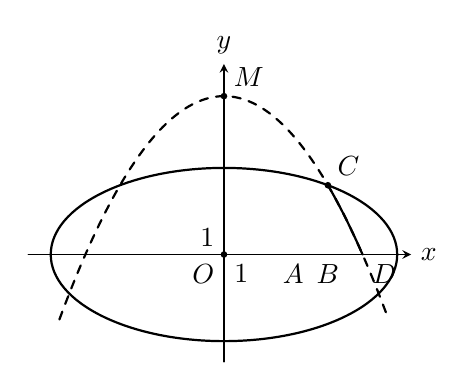
\begin{tikzpicture}[line cap=round,line join=round,x=0.22cm,y=0.22cm,>=stealth]
  % 坐标轴与椭圆运行轨迹 x^2/100+y^2/25=1。
  \draw[->] (-11.3,0)--(10.8,0) node[right] {$x$};
  \draw[->] (0,-6.2)--(0,11.0) node[above] {$y$};
  \draw[thick] (0,0) ellipse (10 and 5);

  % 变轨后的抛物线 y=64/7-x^2/7，原卷以虚线表示。
  \draw[dashed,thick,domain=-9.5:9.5,samples=100,variable=\x]
    plot (\x,{64/7-\x*\x/7});
  % 原卷以实线强调从交点 C 到降落点 D 的运行弧段。
  \draw[thick,domain=6:8,samples=40,variable=\x]
    plot (\x,{64/7-\x*\x/7});

  % 原卷中的基准点与观测点标记。
  \fill (0,0) circle (1.2pt) node[below left] {$O$};
  \fill (0,{64/7}) circle (1.2pt) node[above right] {$M$};
  \fill (6,4) circle (1.2pt) node[above right] {$C$};
  \node[below] at (4,0) {$A$};
  \node[below] at (6,0) {$B$};
  \node[below right] at (8,0) {$D$};
  \node[below] at (1,0) {$1$};
  \node[left] at (0,1) {$1$};
\end{tikzpicture}
